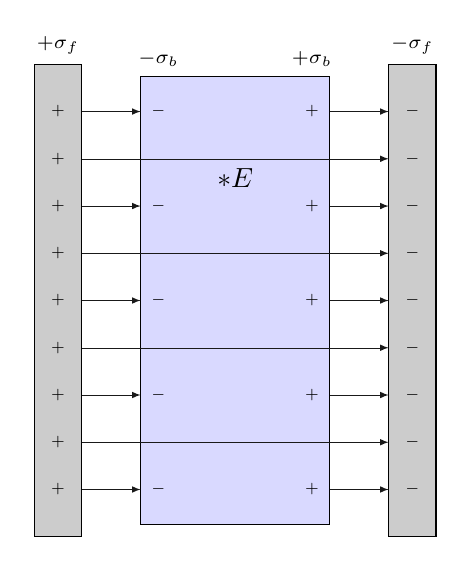
\begin{tikzpicture}[scale=1.5]
    \draw[fill=black,fill opacity=0.2] (-1.7,-2) rectangle (-1.3,2);
    \draw[fill=black,fill opacity=0.2] (+1.7,-2) rectangle (+1.3,2);
    \draw[fill=blue,fill opacity=0.15] (+0.8,-1.9) rectangle (-0.8,1.9);
    \node[above] at (+1.5,2) {\scriptsize $-\sigma_f$};
    \node[above] at (-1.5,2) {\scriptsize $+\sigma_f$};
    \node[above] at (+0.65,1.9) {\scriptsize $+\sigma_b$};
    \node[above] at (-0.65,1.9) {\scriptsize $-\sigma_b$};
    \foreach \x in {1.6,1.2,...,-1.61}
    {
        \node at (+1.5,\x) {\tiny $-$};
        \node at (-1.5,\x) {\tiny $+$};
    }
    \foreach \x in {1.6,0.8,...,-1.61}
    {
        \node at (-0.65,\x) {\tiny $-$};
        \node at (+0.65,\x) {\tiny $+$};
    }
    \foreach \x in {1.2,0.4,...,-1.21}
    {
        \draw[-latex,ultra thin,black!90!white] (-1.3,\x)--(+1.3,\x);
    }
    \foreach \x in {1.6,0.8,...,-1.61}
    {
        \draw[-latex,ultra thin,black!90!white] (-1.3,\x)--(-0.8,\x);
        \draw[-latex,ultra thin,black!90!white] (+0.8,\x)--(+1.3,\x);
    }
    \node[below] at (0,1.2) {$\vb*{E}$};
\end{tikzpicture}
